%-------------------------------------------------------------------------------
% Methoden
%-------------------------------------------------------------------------------
\section{Methoden}

Um herauszufinden, welchen Einfluss die Spielmechaniken Abzeichen und Fortschrittsbalken auf Motivation und Leistung haben, wird eine quantitative Studie in Form eines Onlineexperiments durchgeführt. Das Experiment besteht aus einer interaktiven Konsolenanwendung, die im Browser läuft und das Verhalten einer nativen Kommandozeile möglichst exakt imitiert. Im Rahmen des Experiments wird den Teilnehmern eine vordefinierte Menge an Fragen gestellt, die es durch die Eingabe typischer Konsolenbefehle zu lösen gilt. Die Teilnehmenden werden randomisiert einer der drei Versuchsbedingungen zugeordnet. Die Anwendung ist in ihrer Grundform bewusst demotivierend gestaltet und stellte damit einen spielfremden Kontext dar. Dies geschieht unter der Annahme, dass Aufgaben nur solange bearbeitet werden, wie es den Teilnehmenden Spaß bereitet.

\subsection{Zielgruppe}
Die Zielgruppe besteht aus Personen, die Berührungspunkte mit der Kommandozeile haben oder Interesse an einem Erlernen grundlegender Fähigkeiten eben dieser haben. Die Fragen sind daher so gewählt, dass diese auch durch einen Beginner lösbar sind.
Zusätzlich wird eine optionale Hilfsfunktion integriert, die hilfreiche Tipps für das Lösen der Aufgabe bereitstellt.
Damit zielte die Anwendung u.a. auf informatikaffine Personen, Studenten eines MINT-Faches, Entwickler, Systemadministratoren und Informatiker ab. Die Beschaffenheit der Zielgruppe lässt die Annahme zu, dass die Teilnehmer ausreichende Englischkenntnisse besitzen, um eine englische Anwendung zu bedienen. Daher ist die Anwendung ausschließlich auf Englisch lokalisiert.

\subsection{Versuchsablauf}
Das Experiment findet ausschließlich online statt. Die Teilnahme ist von einem beliebigen Endgerät möglich. Dabei wird bewusst darauf geachtet, dass die Anwendung von mobilen Geräten erreichbar und auch nutzbar ist. Dies geschieht mit der Absicht, die Anzahl potentieller Teilnehmer zu maximieren. Das Experiment ist zu einem beliebigen Zeitpunkt durch den Probanden unterbrechbar. Der Fortschritt wird dann gespeichert und eine Fortsetzung des Experiments ist zu einem späteren Zeitpunkt möglich.

Zu Beginn des Experiments wird jedem Teilnehmer einmalig ein Willkommensbildschirm angezeigt. Auf diesem werden die Teilnehmer auf die Rahmenbedingungen des Experiments hingewiesen. Dazu zählte der Hinweis, dass es sich bei der Anwendung um ein Experiment handelt, ein Verweis auf den Quellcode der Anwendung\footnote{Link: https://github.com/M0r13n/terminal} und eine Verlinkung zur Datenschutzerklärung. Die Teilnehmer werden zusätzlich gebeten, vier Fragen zu beantworten. Dabei handelt es sich um einen Fragebogen, der durch Abhaken von Checkboxen zu beantworten ist. Die Fragen dienen einer grundlegenden demographischen Einordnung der Teilnehmer. Es werden die folgende Fragen gestellt (die Antwortmöglichkeiten sind in Klammern, durch Kommata getrennt dargestellt):

\begin{enumerate}\label{demography}
	 \item \textbf{How old are you (in years)?} (<18, 18-29, 29-39, 39-59, 59+)
     \item \textbf{What is your gender?} (other, female, male)
     \item \textbf{How well would you describe your English skills?} (very good, good, not so good, nonexistent)
     \item \textbf{How often do you use the commandline?} (daily, occasionally (1x per week), rarely (1x per month), very rarely (1x per year or less), I have never used it)
\end{enumerate}

Eine Teilnahme an dem Experiment ist nur nach der erfolgreichen Beantwortung der Fragen möglich. Anschließend wird jede Person zufällig und dauerhaft einer von drei Versuchsbedingungen zugewiesen.


\begin{itemize}
	\item \textbf{Kontrollgruppe:} Probanden der Kontrollgruppe müssen die Fragen ohne motivierende Spielmechaniken beantworten.
	 
    \item \textbf{Experimentalbedingung Abzeichen (EB):} Probanden der Experimentalgruppe Abzeichen erhalten in regelmäßigen Abständen Abzeichen.

    \item \textbf{Experimentalbedingung Fortschrittsanzeige (EP):} Probanden der Experimentalgruppe sehen einen klassischen, horizontalen Fortschrittsbalken am oberen Bildschirmrand.
\end{itemize}

Zu Beginn des Experiments erhalten die Teilnehmenden eine kurze Einweisung. In dieser wird die grundlegende Bedienung und Funktion des Terminals erklärt. Dabei wird explizit auf die besonderen Kommandozeilenbefehle \textbf{clear}, \textbf{about}, \textbf{bug} und \textbf{help} hingewiesen. Die Einweisung wird erneut angezeigt, wenn ein Teilnehmender das Experiment unterbricht und an einem späteren Zeitpunkt fortsetzt.

\paragraph{clear}
Dieser Befehl löscht die Historie der angezeigten Befehle und hinterlässt somit ein sauberes Terminal.

\paragraph{about}
Dieser Befehl führt den Teilnehmer auf eine Infoseite. Auf dieser sind alle Informationen über das Experiment zusammengefasst.

\paragraph{bug}
Dieser Befehl erlaubt es dem Probanden einen Fehlerbericht zu erstellen und abzuschicken.

\paragraph{help}
Dieser Befehl offenbart für jede Frage einen Lösungshinweis. \\

Unter dem Instruktionstext wird die aktuelle Aufgabe präsentiert. Der Rest der Webseite besteht aus einer interaktiven Kommandozeile, die einem klassischen Terminal hinsichtlich Bedienung und Optik gleicht. Nach dem Beenden des Experiments sind die Teilnehmer angehalten, ihre persönliche Einstellung hinsichtlich empfundener Motivation, entsprechend der 5-Stufigen-Lickert-Skala, anzugeben. Konkret wird den Teilnehmenden folgende Frage gestellt:

\begin{description}
\item[Frage]\hfill \\ How much do you agree with the following statement: \textit{I felt motivated in using the application.} ?
\item[Antwortmöglichkeiten]\hfill 


\begin{itemize}
	 \item Strongly disagree (1),
	 \item Disagree (2)
	 \item Neither agree nor disagre (3)
	 \item Agree (4)
	 \item Strongly agree (5)
\end{itemize}
\end{description}


\subsection{Beschreibung der Versuchsbedingungen}
Die Experimentalbedingung Abzeichen erhält eine Leiste am oberen Bildschirmrand, welche fünf Abzeichen beinhaltet. Diese sind zunächst grau hinterlegt, um die Teilnehmenden indirekt auf weitere Abzeichen hinzuweisen. Erst wenn die Bedingungen für das Erreichen des jeweiligen Abzeichens erreicht sind, wird dieses farblich hervorgehoben. Das Erreichen eines Meilensteins wird zudem durch eine Animation begleitet. Dies geschieht unter der Annahme, dass eine optisch ansprechende und auffällige Animation die Motivation der Teilnehmer weiter steigern würde. Die erforderlichen Bedingungen für das Erreichen eines Abzeichens lassen sich durch einen Klick auf das jeweilige Abzeichen einsehen.

Die Abzeichen wurden auf der Basis der Arbeit von \citeauthorwithyear{antin_badges_2011} gestaltet. Jedes Abzeichen erfüllt mindestens eine der fünf, von \citeauthorwithyear{antin_badges_2011} eingeführten, Hauptfunktionen von Abzeichen.

\paragraph{Abzeichen 1:}
Dieses Abzeichen wird für das Lösen der ersten Aufgabe verliehen. So soll der Nutzer auf weitere Abzeichen aufmerksam gemacht werden. Das Abzeichen hat entsprechend eine instruktive Funktion.

\paragraph{Abzeichen 2:}
Dieses Abzeichen wird für das Lösen aller Probleme verliehen und dient primär als Statussymbol.

\paragraph{Abzeichen 3:}
Dieses Abzeichen wird für die Verkettung von mindestens drei Kommandozeilenbefehlen verliehen und weist damit explizit auf die Möglichkeit der Befehlsverkettung hin. Entsprechend erfüllt das Abzeichen eine instruktive Funktion.

\paragraph{Abzeichen 4:}
Dieses Abzeichen wird für die Lösung der letzten Aufgabe verliehen und dient der Bestätigung der erbrachten Leistung des Probanden. Da diese Aufgabe, im Vergleich zu anderen Aufgaben, vergleichsweise schwierig ist, wirkt das Abzeichen zusätzliche als Statussymbol.

\paragraph{Abzeichen 5:}
Dieses Abzeichen wird für den zehnten Fehlversuch vergeben. Der Nutzer soll nicht für sein Scheitern bestraft werden. Stattdessen wird der Versuch belohnt. Dadurch ist der Nutzer angehalten kreative Wege zu finden, um die Aufgaben zu lösen. Das Abzeichen fungiert damit indirekt als Zielvorgabe.


\begin{figure}[htbp]
    \centering
    \includesvg[width = 50pt, height = 50pt]{img/goal.svg}
    \includesvg[width = 50pt, height = 50pt]{img/goal_reached.svg}
    \includesvg[width = 50pt, height = 50pt]{img/solutions.svg}
    \includesvg[width = 50pt, height = 50pt]{img/target.svg}
    \includesvg[width = 50pt, height = 50pt]{img/win.svg}
    \caption{Von links nach rechts lesend: Abzeichen 1 bis 5.}
\end{figure}


Die Experimentalbedingung Fortschrittsbalken sieht einen horizontalen, animierten Fortschrittsbalken. Dieser ist auffällig am oberen Bildschirmrand platziert. Um den Nutzer auf die Forschrittsanzeige aufmerksam zu machen, ist diese bereits zu Beginn des Experiments zu einem Prozent gefüllt und durchgehend animiert. Dabei handelt es sich um eine bestimmte Anzeige, die sich entsprechend des aktuellen Fortschritts des Teilnehmers zunehmend füllt. Somit ist es dem Probanden möglich durch den Füllstand des Fortschrittsbalkens auf die Restdauer des Experiments zu schließen.

Beide Experimentalbedingungen unterscheiden sich ausschließlich hinsichtlich der geschilderten visuellen Elemente. Um die Vergleichbarkeit sicherzustellen, wurden identische Fragen in derselben Reihenfolge abgefragt. Durch die Trennung der einzelnen Spielelemente in unterschiedliche Versuchsbedingungen kann jedes Spielelement individuell beurteilt werden. Auf diese Weise können die Spielelemente Abzeichen und Fortschrittsanzeige individuell auf ihren Einfluss auf Motivation und Leistung untersucht werden.

\begin{figure}[htbp]
    \centering
    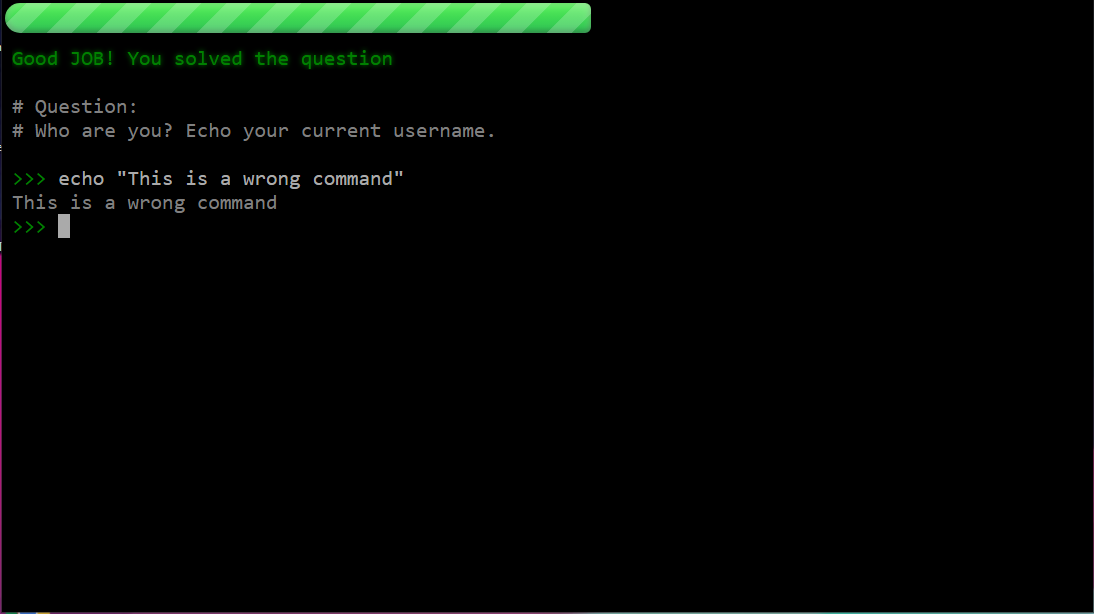
\includegraphics[width=\textwidth]{img/full_web.png}
    \caption{Falsch beantwortete Beispielfrage in der Experimentalbedingung 'Fortschrittsanzeige'.}
\end{figure}

\subsubsection{Technische Implementation}
Bei der entwickelten Anwendung handelt es sich um eine interaktive Webanwendung. Diese ist sowohl auf Mobilgeräten als auch an einem klassischen Computer nutzbar. Die Anwendung besteht aus drei Komponenten: Einer statischen Webseite, einem Server und einem Executor. 

\paragraph{Statische Webseite:}
Die Webseite basiert auf HTML, CSS und Javascript. Die graphische Darstellung einer Kommandozeile basiert auf dem jQuery Plugin \qq{jQuery Terminal Emulator}\footnote{https://terminal.jcubic.pl/}. Die Webseite kommuniziert über eine REST-API mit dem Server. Über diese Schnittstelle werden Nutzerdaten und abgesetzte Befehle kommuniziert. Die Webseite verfügt über keinerlei Anwendungslogik und stellt lediglich die empfangenen Daten des Servers graphisch dar. Für die gesamte Anwendung wurde ein dunkles Farbschema gewählt. Dieses besteht im Kern aus den Farben Grün und Schwarz und ähnelt damit einem typischen Terminal.

\paragraph{Server:}
Der Server ist in Python geschrieben und basiert auf dem verbreiteten Framework \qq{Flask}\footnote{https://github.com/pallets/flask}. Der Server ist verantwortlich für die Nutzerverwaltung, die Nutzererkennung, das Ausführen und die anschließende Validierung abgesetzter Befehle sowie die Datenerfassung. Sämtliche Daten werden in einer MySQL-Datenbank gespeichert. Empfangene Befehle reicht der Server an den Executor weiter. Die Kommunikation erfolgt auch hier über eine JSON-basierte REST-API. Der Server fungiert zusätzlich als Cache für bereits ausgeführte Befehle. Diese werden in der Datenbank zwischengespeichert. Somit muss jeder Befehl nur ein einziges Mal real ausgeführt werden.

\paragraph{Executor:}

  Da Konsolenbefehle kombinierbar sind, gibt es mehrere Antwortmöglichkeiten für ein und dieselbe Frage. Selbst einfache Fragen wie \textit{Geben Sie \say{Hello World} auf der Kommdozeile aus} haben nahezu unendlich viele Lösungsmöglichkeiten. Mögliche Antwortmöglichkeiten sind etwa 
  \begin{center}
      \verb|echo Hello World|
  \end{center}
  oder 
   \begin{center}
      \verb|echo hello world > t && cat t|.
  \end{center}
  Daher ist es nötig, die abgesendeten Befehle real auszuführen. Dazu wird jeder Befehl in einem eigenen Docker Container ausgeführt und die Ausgabe sowie mögliche Seiteneffekte mit der erwarteten Ausgabe abgeglichen. Diese Aufgabe übernimmt der Executor als separate Komponente. Dabei handelt es sich um eine simple Python API. Diese ist verantwortlich für das Starten, Verwalten und Löschen von Dockercontainern. Für jeden Befehl wird ein neuer Container gestartet und die Ausgabe des Befehls auf ihre Korrektheit überprüft. Die Container basieren auf einem minimalen Python Image. 


\subsubsection{Datenerfassung}
Während des Experiments wurden unterschiedliche Daten erfasst. Diese Daten dienen sowohl der Auswertung und Analyse des Experiments als auch dem Ausschluss von Mehrfachteilnahmen. Die folgenden Daten wurden für jeden Probanden gespeichert.

\paragraph{Demographische Daten:}
Die in \ref{demography} dargestellten Fragen wurden für jeden Nutzer in der Nutzertabelle gespeichert. Zusätzlich wurde die jeweilige Experimentalbedingung in derselben Tabelle gespeichert.

\paragraph{Gerätespezifische Daten:}
Für jeden Nutzer wurde die IP-Adresse sowie der User-Agent gespeichert. Auf diese Weise sollen Mehrfachteilnahmen des gleichen Nutzers ausgeschlossen werden.

\paragraph{Nutzungsdaten:}
Während des Experiments wurden unterschiedliche Daten erfasst. Diese Erfassung diente der späteren Bewertung der Effektivität der einzelnen Maßnahmen. Folgende Daten wurden erfasst:

\begin{itemize}
	 \item Abgesendete Befehle mit Zeitstempel
	 \item Gelöste Aufgaben 
	 \item Erreichte Abzeichen (nur für die Experimentalbedingung Abzeichen)
	 \item Feedback hinsichtlich der empfundenen Motivation (nur nach vollständiger Bearbeitung des Experiments)
\end{itemize}


\subsection{Pretest}\label{verlauf}
Vor der Veröffentlichung des Experiments wurde ein Pretest durchgeführt. Durch diesen sollten potentielle Fehler und Unklarheiten im Studiendesign reduziert werden. Zusätzlich konnte überprüft werden, ob die Studie grundlegend funktioniert. Im Rahmen des Tests wurden neben kleineren Fehlern wesentliche Probleme deutlich. Zum einen waren die Abzeichen deutlich zu unauffällig und wirkten laut Aussage der Teilnehmer wenig bis gar nicht motivierend. Aus diesem Grund wurden die Abzeichen größer und farbenfroher gestaltet. Zusätzlich wurde eine Animation abgespielt, sobald ein Abzeichen erreicht wurde. Außerdem gaben mehrere Teilnehmer an, dass die Fragen unverständlich und zu komplex seien. Dies hat dazu geführt, dass die Komplexität der Fragen reduziert wurde. Die so entstandenen Fragen lassen sich durch die Kombination von maximal zwei Befehlen lösen. Zusätzlich wurde eine Hilfsfunktion eingebaut. Durch den Befehl \textbf{help} erhielten Probanden weiterführende Informationen, die der Lösung der Aufgabe dienten. Außerdem wurde die Reaktionszeit der Anwendung (Zeitspanne zwischen dem Absetzen eines Befehls und der Anzeige des Ergebnisses) als zu langsam empfunden. Daher wurde das Image des Containers verkleinert und auf die nötigsten Programme reduziert. Zusätzlich wurde ein Cache für bereits ausgeführte Befehle eingeführt. Auf diese Weise konnte eine Reaktionszeit von 0.5 bis 2 Sekunden pro abgesetztem Befehl gewährleistet werden.


\subsection{Statistische Auswertung}
Leistung messe ich durch die Anzahl beantworteter Fragen. Zusätzlich wird die Gesamtzeit als Vergleichsparameter herangezogen. Diese ergibt sich aus der Differenz des ersten und letzten abgeschickten Befehls. Zeitspannen von mehr als 30 Minuten ohne Nutzeraktivität (d.h. es wurde in einem Zeitraum von 30 Minuten kein Befehl abgesetzt) werden als Inaktivität gewertet und von der Gesamtzeit abgezogen. Dies geschieht unter der Annahme, dass motivierte Teilnehmer mehr Zeit investieren als die Kontrollgruppe. Auf diese Weise wird der Effekt der unabhängigen Variablen Fortschrittsbalken und Abzeichen auf Motivation und Leistung quantifizierbar gemacht. Die aufgestellten Hypothesen werden mithilfe von t-Tests überprüft. Die dafür erforderlichen Voraussetzungen sind erfüllt. Die t-Tests werden durch eine einfaktorielle ANOVA Varianzanalyse erweitert. Durch diese lassen sich die drei Versuchsgruppen miteinander vergleichen.